\documentclass[12pt]{article}
\usepackage{graphicx}
\graphicspath{ {./images/} }
\usepackage[utf8]{inputenc}
\usepackage{amsthm,xpatch}
\usepackage{amsmath}
\usepackage{tikz} 
\usepackage{geometry}
\usepackage{amssymb}
\usepackage{enumerate}
\usetikzlibrary{arrows, automata, calc, positioning}
\geometry{margin=2cm}

\title{MLCS - Homework 2}
\author{Michele Conti \\ \texttt{1599133}}
\date{}


\theoremstyle{definition}
\newtheorem{exerciseinner}{Exercise}
\newenvironment{exercise}[1]{%
	\renewcommand\theexerciseinner{#1}%
	\exerciseinner
}{\endexerciseinner}

\renewcommand*{\proofname}{Solution}

\makeatletter
\newcounter{proofpart}
\xpretocmd{\proof}{\setcounter{proofpart}{0}}{}{}
\newcommand{\proofpart}[1]{%
	\par
	\addvspace{\medskipamount}%
	\stepcounter{proofpart}%
	\noindent\emph{Part \theproofpart: #1}\par\nobreak\smallskip
	\@afterheading
}
\makeatother

\begin{document}
\maketitle

\section{EF-games and (non)-expressibility}

\begin{exercise}{1.6}
	Consider the following two graphs:
	\begin{enumerate}
		\item $\mathfrak{G}_1$ is a line of length $4n$;
		\item $\mathfrak{G}_2$ consists of a line of length $2n$ and a cycle of length $2n$ (the two components are disjoint).
	\end{enumerate}
	Analyze the EF games on these structures for $n = 1, 2$ and write a sentence of minimal quantifier rank distinguishing the two structures for $n = 1, 2$.
	
	BONUS: Formulate a generalization of your observations and prove that the Acyclicity query is not expressible in the language of graphs over finite graphs, using EF-games.
\end{exercise}
\begin{proof}
Let's discuss every point separately.
\proofpart{$n = 1$.}
For $n = 1$, $\mathfrak{G}_1$ is a line of length $4$, while $\mathfrak{G}_2$ is the disjoint structure composed by a line of length $2$ and a cycle of length $2$.
\begin{figure}[h]
	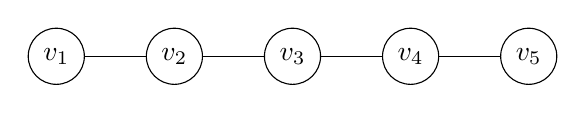
\begin{tikzpicture}[node distance={15mm}, main/.style = {draw, circle}]
		\node[main] (1) {$v_1$};
		\node[main] (2) [right of=1] {$v_2$};
		\node[main] (3) [right of=2] {$v_3$};
		\node[main] (4) [right of=3] {$v_4$};
		\node[main] (5) [right of=4] {$v_5$};
		\draw (1) -- (2);
		\draw (2) -- (3);
		\draw (3) -- (4);
		\draw (4) -- (5);
	\end{tikzpicture}
	\centering
	\caption{Graph $\mathfrak{G}_1$, consisting of a line of length $4$.}
\end{figure}
\begin{figure}[H]
	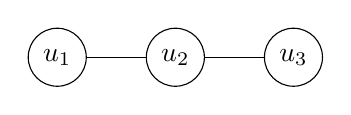
\begin{tikzpicture}[node distance={15mm}, main/.style = {draw, circle}]
		\node[main] (1) {$u_1$};
		\node[main] (2) [right of=1] {$u_2$};
		\node[main] (3) [right of=2] {$u_3$};
		\draw (1) -- (2);
		\draw (2) -- (3);
	\end{tikzpicture}
	\hspace{3cm}
	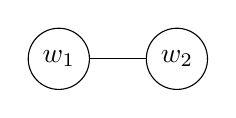
\begin{tikzpicture}[node distance={15mm}, main/.style = {draw, circle}]
		\node[main] (1) {$w_1$};
		\node[main] (2) [right of=1] {$w_2$};
		\draw (1) -- (2);
	\end{tikzpicture}
	\centering
	\caption{Graph $\mathfrak{G}_2$, consisting of a line of length $2$ and cycle of length $2$.}
\end{figure}

\proofpart{$n = 2$.}
For $n = 2$, $\mathfrak{G}_1$ is a line of length $8$, while $\mathfrak{G}_2$ is the disjoint structure composed by a line of length $4$ and a cycle of length $4$.
\begin{figure}[H]
	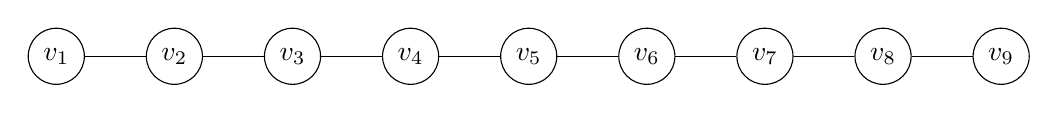
\begin{tikzpicture}[node distance={15mm}, main/.style = {draw, circle}]
		\node[main] (1) {$v_1$};
		\node[main] (2) [right of=1] {$v_2$};
		\node[main] (3) [right of=2] {$v_3$};
		\node[main] (4) [right of=3] {$v_4$};
		\node[main] (5) [right of=4] {$v_5$};
		\node[main] (6) [right of=5] {$v_6$};
		\node[main] (7) [right of=6] {$v_7$};
		\node[main] (8) [right of=7] {$v_8$};
		\node[main] (9) [right of=8] {$v_9$};
		\draw (1) -- (2);
		\draw (2) -- (3);
		\draw (3) -- (4);
		\draw (4) -- (5);
		\draw (5) -- (6);
		\draw (6) -- (7);
		\draw (7) -- (8);
		\draw (8) -- (9);
	\end{tikzpicture}
	\centering
	\caption{Structure $\mathfrak{G}_1$, consisting of a line of length $8$.}
\end{figure}
\begin{figure}[H]
	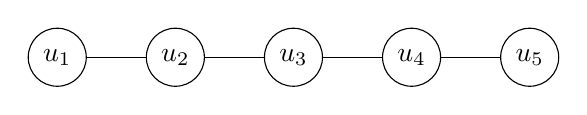
\begin{tikzpicture}[node distance={15mm}, main/.style = {draw, circle}]
		\node[main] (1) {$u_1$};
		\node[main] (2) [right of=1] {$u_2$};
		\node[main] (3) [right of=2] {$u_3$};
		\node[main] (4) [right of=3] {$u_4$};
		\node[main] (5) [right of=4] {$u_5$};
		\draw (1) -- (2);
		\draw (2) -- (3);
		\draw (3) -- (4);
		\draw (4) -- (5);
	\end{tikzpicture}
	\hspace{3cm}
	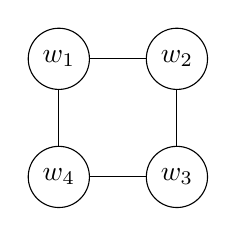
\begin{tikzpicture}[node distance={15mm}, main/.style = {draw, circle}]
		\node[main] (1) {$w_1$};
		\node[main] (2) [right of=1] {$w_2$};
		\node[main] (3) [below of=2] {$w_3$};
		\node[main] (4) [left of=3] {$w_4$};
		\draw (1) -- (2);
		\draw (2) -- (3);
		\draw (3) -- (4);
		\draw (4) -- (1);
	\end{tikzpicture}
	\centering
	\caption{Structure $\mathfrak{G}_2$, consisting of a line of length $4$ and cycle of length $4$.}
\end{figure}
\end{proof}

\end{document}
